\section{Staff Usage}
\label{sec:staff_usage}
The \astaff[] members main usage of the is to solve problems.
This is corresponding to the \ucsolproblem{} use case in section \ref{sec:usecase}.
This use case is how ever quite large, so it is divided into three steps; choosing a problem to solve, communicate with the subscriber(s), solve the problem.
The communication with the subscriber(s) step might not be applied during the solve usage of the \aclient[].
The three steps are described in the following subsections.

\subsection{Choosing a Problem to Solve}
\begin{figure}[htb]
	\centering
		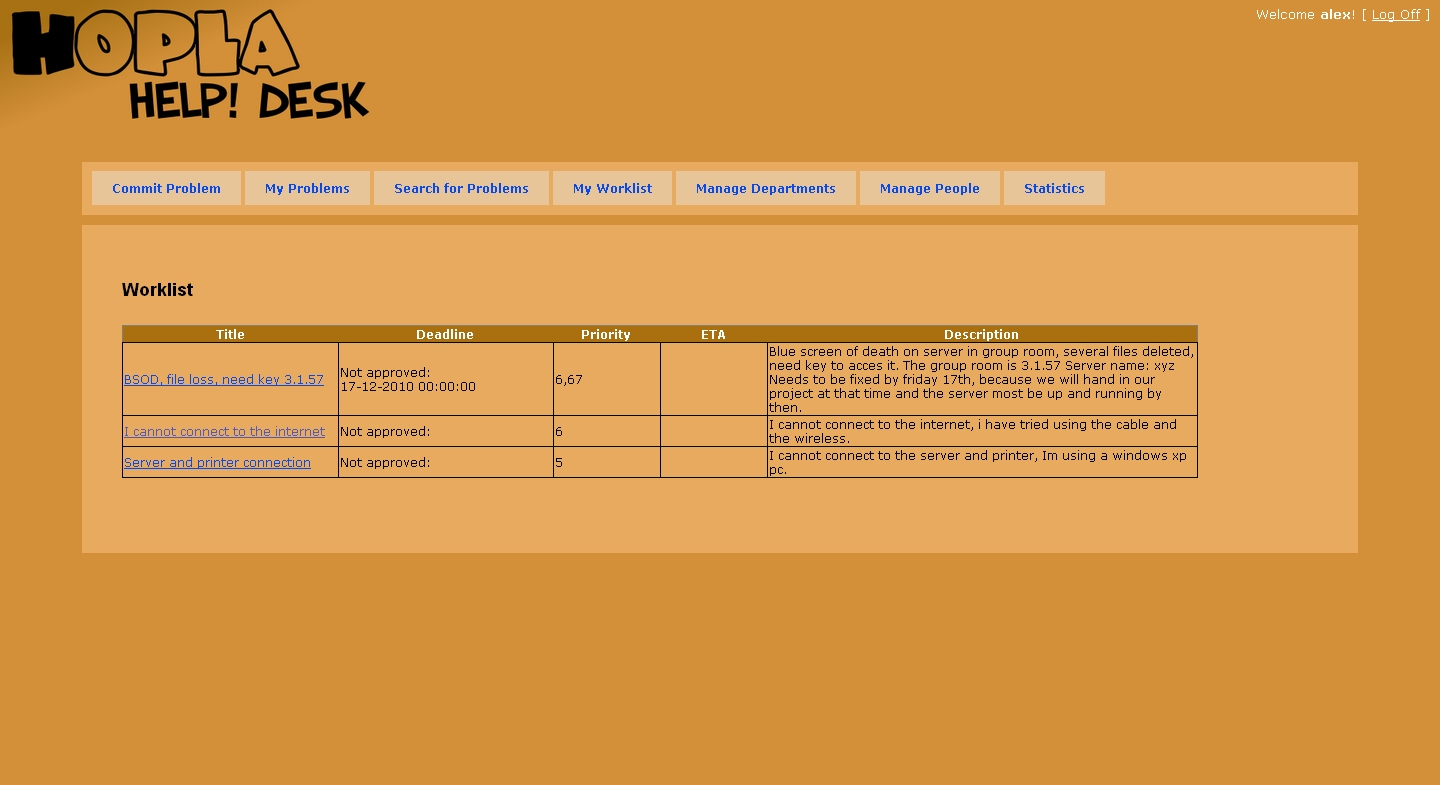
\includegraphics[width=1.00\textwidth, clip=true, trim=4cm 10.5cm 8cm 8cm]{input/implementation/program_presentation/worklist.png}
	\morscaption{A \astaff[] members worklist}
	\label{fig:worklist}
\end{figure}

When a \astaff[] member wants to solve a problem he/she clicks the menu point called My Worklist which can be seen in figure \ref{fig:master}.
This shows the worklist of current logged in \astaff[] user.
An example of a worklist is shown in figure \ref{fig:worklist}.
The \astaff[] member can see the title, description, deadline, priority, and ETC.
He/she can click on a problem in order to get a more detailed view of that specific problem.
The \astaff[] members are responsible for choosing the right problems in the right order them selves, but they can use the priority as a guideline for which problems should be solved first.
This is made easier by the system because the list of problems is ordered by the priority of the problems.


\begin{figure}[htb]
	\centering
		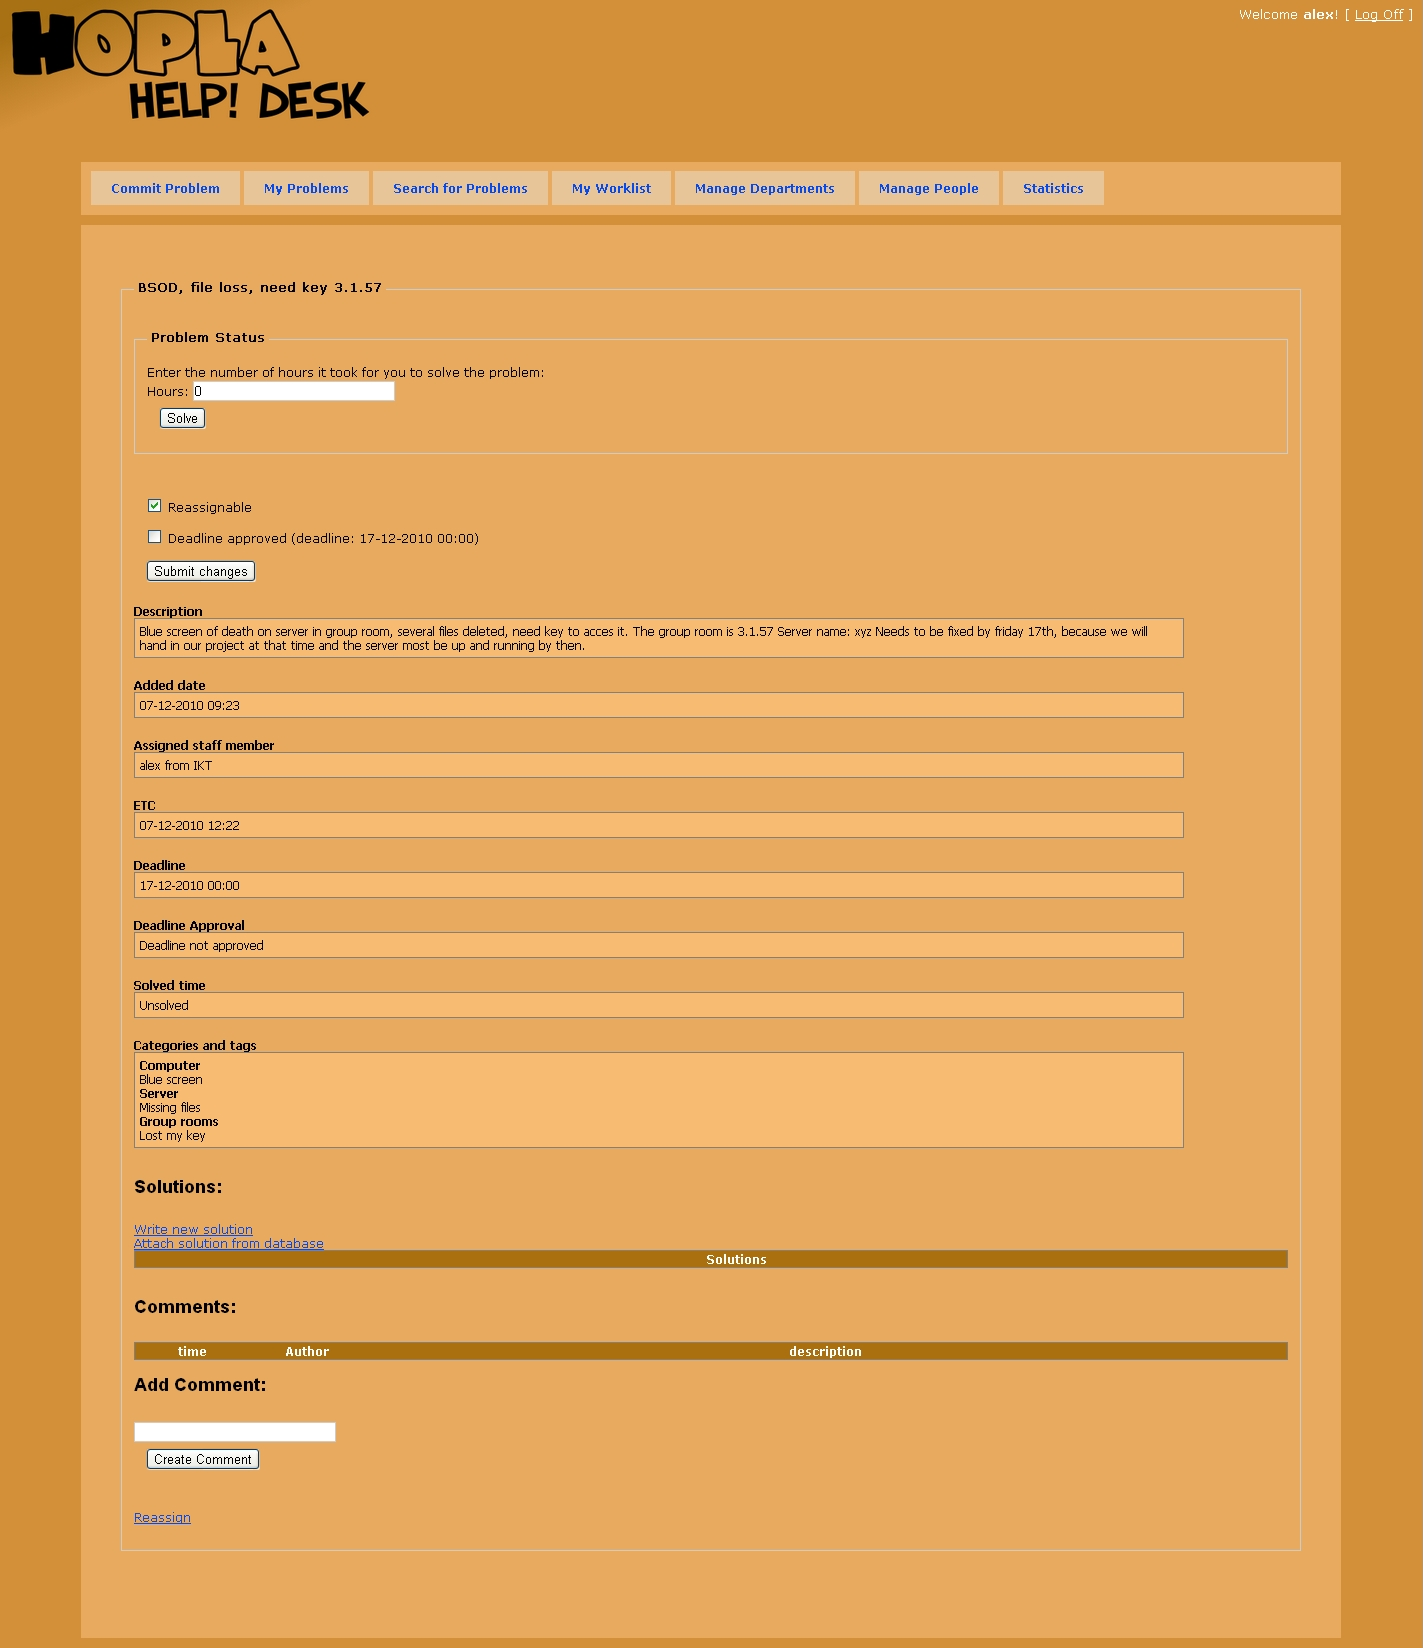
\includegraphics[width=1.00\textwidth, clip=true, trim=3cm 0.5cm 3cm 8cm]{input/implementation/program_presentation/staffProbDetails.png}
	\morscaption{A \astaff[] members problem details view}
	\label{fig:staffProbDetails}
\end{figure}

It is from problem details view that the \astaff[] member can communicate with the subscribers, accept the deadline, lock the problem to him/her self, attach solutions, and finally declare the problem solved.
Even though this view share name with the problem details that a client can access, the \astaff[] members do have more options, as described above.
The \astaff[] members problem details view can be seen in figure \ref{fig:staffProbDetails}.
To accept the deadline a \astaff[] member simply checks a check box and submit the change.
When a \staff[] member has chosen problem to start working on, he/she can make it non-reassignable by unchecking the reassignable check box.
This will stop the balance workload function, which is described in section \ref{sec:balanceworkload}, from removing that given problem from the \astaff[] member while he/she is working on it.
If the \astaff[] member does not do this, the problem might be reassigned to another \astaff[] member and thereby reducing the effectiveness of the recourses because to \astaff[] members will be work on the same problem.

The \astaff[] members can reassign problems which have been assigned to them.
When doing so, he/she can either reassign directly to another \astaff[] member or to a department.
In either case the problem will be marked non-reassignable, in order to stop the balance workload function from moving it to another \astaff[] member or back to the \astaff[] member who had it in the first place.

\subsection{Communicate With Subscribers}
To communicate with the subscribers, the \astaff[] member can write comments to a problem, which the subscribers can see and again respond to.
This communication is important because the \astaff[] member might need more details about a problem in order to solve it.

\subsection{Solve the Problem}
Through the \staff[] members problem details it is possible to attach an existing solution or write a new one.
Once a problem has been given a solution the subscribers are notified and they can check if the solution actually solved their problem.
They can then write a comment back telling the assigned \astaff[] member whether or not the solution solved the problem for them.
If the subscribers are content with the solution(s) the \astaff[] member can mark the problem as solved and enter the time he spend on the problem, so that future problems similar to the given can be given an estimation.

If a \astaff[] member wants to use an already existing solution he will have to search the database for it.
Here is used a search view very similar to the one which the \aclient[]s have, which is described in subsection \ref{sub:searchUsage}.
The difference is that the \astaff[] does not have the opportunity to choose any of the following options: Only my problems, only solved problems, only unsolved problems, and minimum number of problems.
The reason for this is to make it simpler and faster to find the solution.
When the \astaff[] member finds a problem with the right solution, he/she can attach this to the problem currently being solved.

To write a new solution the \astaff[] member clicks the corresponding link in the \astaff[]s problem details view.
He/she is then presented with a text area and a create button.
When the button is clicked, a new solution is created with the given text is attached to the problem being solved.
The problem is not marked as solved as soon as a solution is attached to it, because the solution might not actually have solved the problem or the \astaff[] member might want to attach more than one solution before he/she wants to mark it solved.
